\documentclass{beamer}[10]

\usepackage{graphicx}
\usepackage{xcolor}
\usepackage{tabto}
%\usepackage{beamerthemesplit}
\usepackage{tikz}
\usepackage{cancel}
\usepackage{verbatim}
\usepackage{fancybox}
\usepackage{enumerate}
\usepackage{amsmath,amssymb,amsthm,textcomp,mathtools}
\usepackage[super]{nth}
\usepackage[amssymb]{SIunits}
\usepackage{booktabs}
\usepackage{cancel}
\usepackage{bm}
\usepackage[utf8]{inputenc}
\usepackage{tabularx}
\usepackage{ragged2e}
\newcolumntype{Y}{ >{\RaggedRight\arraybackslash}X}
\usetikzlibrary{arrows,shapes}
\newcommand\T{\rule{0pt}{2.6ex}}
\newcommand\B{\rule[-1.2ex]{0pt}{0pt}}
\definecolor{UUcrimson}{RGB}{204,0,0}
\mode<presentation>
{ \usetheme{default}
  \usecolortheme[named=UUcrimson]{structure}
  \useinnertheme{circles}
  \setbeamercovered{transparent}
  \setbeamertemplate{blocks}[rounded]
  \usefonttheme[onlymath]{serif}
  \setbeamertemplate{navigation symbols}{}
  \setbeamertemplate{footline}[page number]
  \setbeamertemplate{navigation symbols}{}
  \setbeamercolor{section in toc}{fg=black,bg=white}
  \setbeamercolor{alerted text}{fg=UUcrimson!80!gray}
  \setbeamercolor*{palette primary}{fg=white,bg=UUcrimson}
  \setbeamercolor*{palette secondary}{fg=UUcrimson!70!black,bg=gray!15!white}
  \setbeamercolor*{palette tertiary}{bg=UUcrimson!80!black,fg=gray!10!white}
  \setbeamercolor*{palette quaternary}{fg=UUcrimson,bg=gray!5!white}
  \setbeamercolor*{palette sidebar primary}{fg=UUcrimson!10!black}
  \setbeamercolor*{palette sidebar secondary}{fg=white}
  \setbeamercolor*{palette sidebar tertiary}{fg=UUcrimson!50!black}
  \setbeamercolor*{palette sidebar quaternary}{fg=gray!10!white}
  \setbeamercolor{titlelike}{parent=palette primary,fg=white}
  \setbeamercolor{frametitle}{bg=UUcrimson}
  \setbeamercolor{frametitle right}{bg=UUcrimson}
  \setbeamercolor*{separation line}{}
  \setbeamercolor*{fine separation line}{}
}

\usetikzlibrary{backgrounds}
\makeatletter
\tikzstyle{every picture}+=[remember picture]
\tikzset{%
  fancy quotes/.style={
    text width=\fq@width pt,
    align=justify,
    inner sep=1em,
    anchor=north west,
    minimum width=\linewidth,
    font=\itshape
  },
  fancy quotes width/.initial={.8\linewidth},
  fancy quotes marks/.style={
    scale=8,
    text=white,
    inner sep=0pt,
  },
  fancy quotes opening/.style={
    fancy quotes marks,
  },
  fancy quotes closing/.style={
    fancy quotes marks,
  },
  fancy quotes background/.style={
    show background rectangle,
    inner frame xsep=0pt,
    background rectangle/.style={
      fill=gray!25,
      rounded corners,
    },
  }
}
\newenvironment{fancyquotes}[1][]{%
\noindent
\tikzpicture[fancy quotes background]
\node[fancy quotes opening,anchor=north west] (fq@ul) at (0,0) {``};
\tikz@scan@one@point\pgfutil@firstofone(fq@ul.east)
\pgfmathsetmacro{\fq@width}{\linewidth - 2*\pgf@x}
\node[fancy quotes,#1] (fq@txt) at (fq@ul.north west) \bgroup}
{\egroup;
\node[overlay,fancy quotes closing,anchor=east] at (fq@txt.south east) {''};
\endtikzpicture}
\makeatother


\usetikzlibrary{backgrounds}
\makeatletter
\tikzstyle{every picture}+=[remember picture]
\tikzset{%
  fancy defs/.style={
    text width=\fq@width pt,
    align=justify,
    inner sep=0.25em,
    anchor=north west,
    minimum width=\linewidth,
    font=\itshape
  },
  fancy defs width/.initial={.8\linewidth},
  fancy defs marks/.style={
    scale=8,
    text=white,
    inner sep=0pt,
  },
  fancy defs opening/.style={
    fancy defs marks,
  },
  fancy defs closing/.style={
    fancy defs marks,
  },
  fancy defs background/.style={
    show background rectangle,
    inner frame xsep=0pt,
    background rectangle/.style={
      fill=gray!25,
      rounded corners,
    },
  }
}
\newenvironment{fancydefs}[1][]{%
\noindent
\tikzpicture[fancy defs background]
\node[fancy defs opening,anchor=north west] (fq@ul) at (0,0) {};
\tikz@scan@one@point\pgfutil@firstofone(fq@ul.east)
\pgfmathsetmacro{\fq@width}{\linewidth - 2*\pgf@x}
\node[fancy defs,#1] (fq@txt) at (fq@ul.north west) \bgroup}
{\egroup;
\node[overlay,fancy defs closing,anchor=east] at (fq@txt.south east) {};
\endtikzpicture}
\makeatother
\usepackage{scalerel}[2014/03/10]
\usepackage{stackengine}
\usepackage{empheq}
\newcommand*\widefbox[1]{\fbox{\hspace{0.5em}#1\hspace{0.5em}}}

\newcommand\reallywidetilde[1]{\ThisStyle{%
  \setbox0=\hbox{$\SavedStyle#1$}%
  \stackengine{-.1\LMpt}{$\SavedStyle#1$}{%
    \stretchto{\scaleto{\SavedStyle\mkern.2mu\sim}{.5467\wd0}}{.4\ht0}%
%    .2mu is the kern imbalance when clipping white space
%    .5467++++ is \ht/[kerned \wd] aspect ratio for \sim glyph
  }{O}{c}{F}{T}{S}%
}}
\usepackage{media9}

\logo{
\includegraphics[width=0.75cm]{logo.jpg}}
\author[Gibbs]{Dr. Jeremy A. Gibbs}
\institute{Department of Mechanical Engineering\\University of Utah}
\date{Spring 2017}
\title{Environmental Fluid Dynamics: Radiation Model}
% colors
\definecolor{colororange}{HTML}{E65100} % orange
\definecolor{colordgray}{HTML}{795548} % dark gray for note
\definecolor{colorhgray}{HTML}{212121} % heavy dark gray for normal text
\definecolor{colorgreen}{HTML}{009688} % green
\definecolor{colorwhite}{HTML}{FFFFFF} % background white
\definecolor{colorlgray}{HTML}{F5F3EE} % background light gray
\definecolor{colorblue}{HTML}{0277BB} % blue
\definecolor{colorred}{HTML}{CC0000} % red
\newcommand{\fontsizeone}{1.9em}
\setbeamertemplate{caption}{\raggedright\insertcaption\par}
\newcommand{\framecard}[2][colorgreen]{
  {\setbeamercolor{background canvas}{bg=#1}
    \begin{frame}[plain]
    \vfill
    \begin{center}
     {#2}
    \end{center}
    \vfill
    \end{frame}
  }
}

\begin{document}

%----------------------------------------------------------------------------------------
%	TITLE & TOC SLIDES
%----------------------------------------------------------------------------------------

\begin{frame} 
  \titlepage
\end{frame}

%------------------------------------------------

\begin{frame}
\frametitle{Overview}
\tableofcontents
\end{frame}

%------------------------------------------------
\section{A Simple Model for the Computation of Radiation on a Slope} %
%------------------------------------------------
\framecard[colorred]{{\color{white}\Huge A Simple Model for the Computation of Radiation on a Slope}}
%------------------------------------------------
\subsection{Overview}
%------------------------------------------------

\begin{frame}{Radiation Model: Overview}
\begin{figure}
	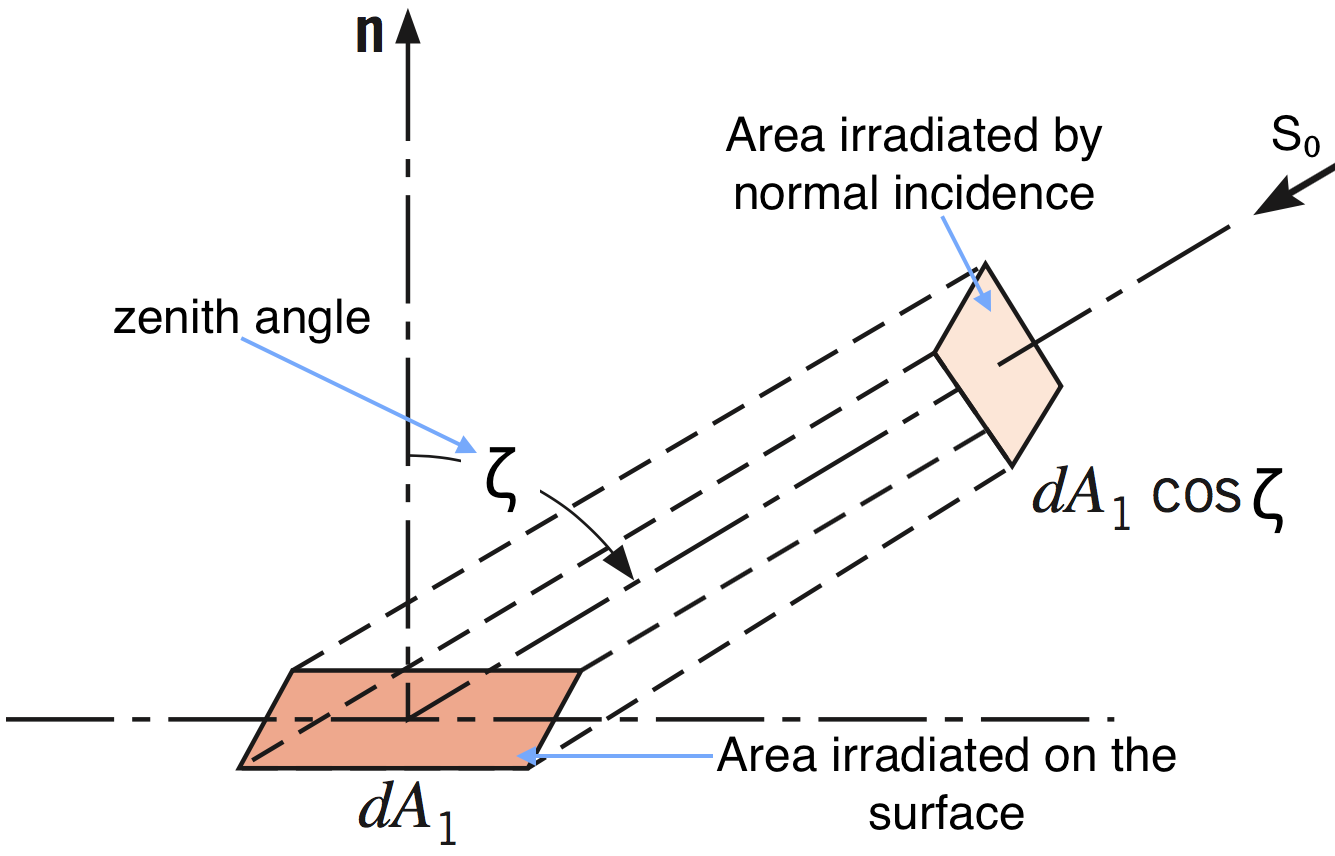
\includegraphics[width=0.85\textwidth]{fig3}
\end{figure}
\begin{itemize}
	\item Flux density on a horizontal surface
	$$S=S_0 \cos \zeta \rightarrow \text{Lambert's Cosine Law}$$
	where $S_0 = 1367\ \watt\ \metre\rpsquared$ is the solar constant
\end{itemize}
\end{frame}

%------------------------------------------------

\begin{frame}{Radiation Model: Overview}
\textbf{We want to consider a more general case of radiation on a slope of arbitrary}:
\begin{itemize}
	\item angle
	\item orientation
	\item time of day
	\item location on Earth
	\item time of year 
\end{itemize}
\textbf{Let's build a model}:
\begin{itemize}
	\item Consider seasonal effects (Earth's orbit)
	\item Daily effects (local sun angle and azimuth)
	\item Slope (mountains, walls, etc)
	\item Atmospheric composition
\end{itemize}
\end{frame}

%------------------------------------------------
\subsection{Seasonal Effects}
%------------------------------------------------
\begin{frame}{Radiation Model: Seasonal Effects}
\begin{columns}[T]
    \begin{column}{.5\textwidth}
    \begin{minipage}[c][0.7\textheight][c]{\linewidth}
    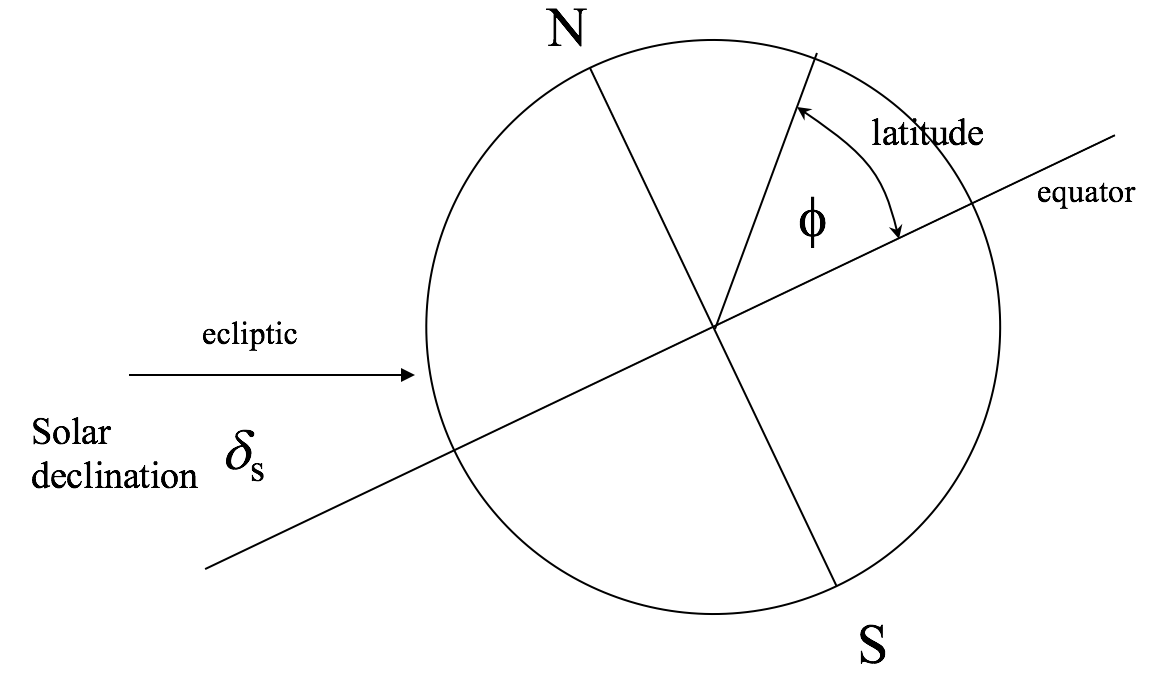
\includegraphics[width=1\textwidth]{fig4}\\
    \end{minipage}
    \end{column}
    \begin{column}{.5\textwidth}
    \begin{minipage}[c][0.65\textheight][c]{\linewidth}
   \begin{itemize}
   	\item $\phi$ - latitude
   	\item $\phi_r$ - tilt of the Earth's axis relative to the ecliptic (orbital plane of the Earth around the sun)
   	\item $\phi_r = 23.45^\circ = 0.409\ \radian$ corresponds to the latitude of the tropics (Capricorn and Cancer)
   \end{itemize}
      \end{minipage}
    \end{column}
  \end{columns}
\end{frame}
%------------------------------------------------
\begin{frame}{Radiation Model: Seasonal Effects}
\begin{columns}[T]
    \begin{column}{.5\textwidth}
    \begin{minipage}[c][0.7\textheight][c]{\linewidth}
    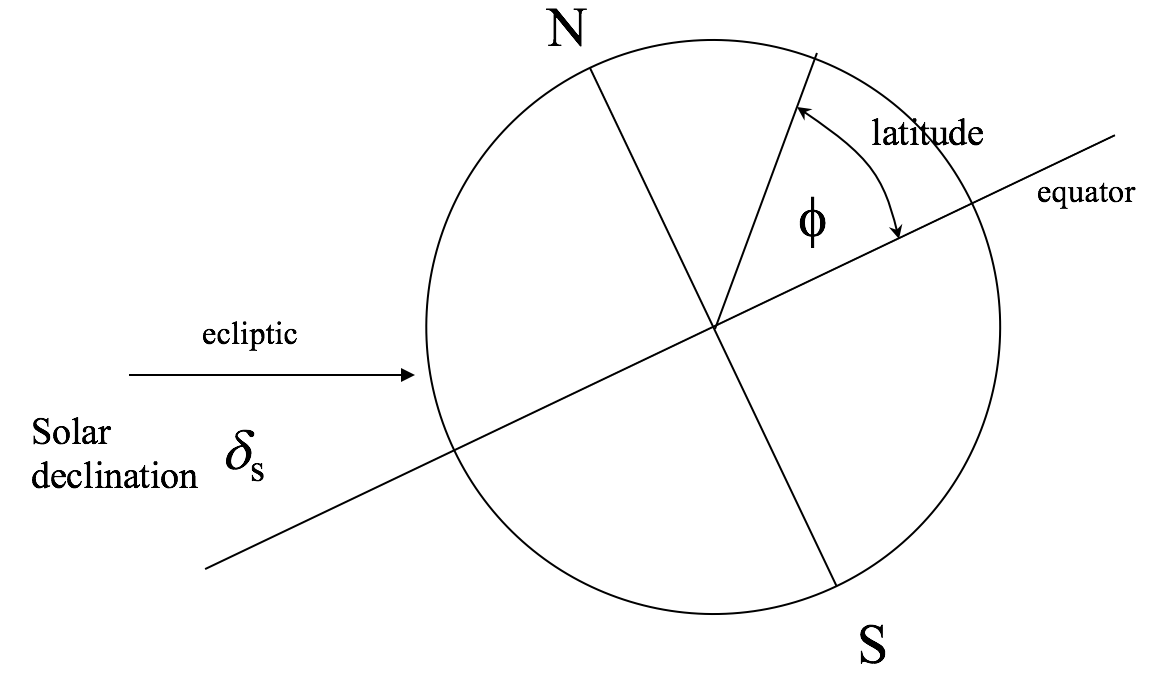
\includegraphics[width=1\textwidth]{fig4}\\
    \end{minipage}
    \end{column}
    \begin{column}{.5\textwidth}
    \begin{minipage}[c][0.65\textheight][c]{\linewidth}
   \textbf{Solar declination} $\delta_s$
   \begin{itemize}
   	\item Angle between the ecliptic and the equator as the Earth rotates around the sun
   	\item Summer and Winter
   	$$\underbrace{-23.45^\circ}_{\text{winter solstice}} \lesssim \delta_s \lesssim \underbrace{23.45^\circ}_{\text{summer solstice}}$$
   	\item Spring and Autumn\\
   	$\delta_s=0$ means sun is directly overhead at equator: equinox \\vernal  (Mar 19-21) autumnal (Sept 22-24)
   \end{itemize}
      \end{minipage}
    \end{column}
  \end{columns}
\end{frame}
%------------------------------------------------
\begin{frame}{Radiation Model: Seasonal Effects}
\textbf{Solar declination} $\delta_s$
\begin{itemize}
	\item For a circular orbit:
	$$\delta_s = \phi_r \cos \left[\frac{C(d-d_r)}{d_y}\right]$$
	where
	\begin{itemize}
		\item $C=360^\circ$ or $2\pi\ \radian$
		\item $d =$ day of the year (Julian date 1-365, or 366)
		\item $d_r =$ summer solstice (June 22, 173 JD, 20-22)
		\item $d_y =$ 365 or 366 days
		\item $\phi_r =$ tilt of Earth's axis relative to the ecliptic ($23.45^\circ$)
	\end{itemize}
\end{itemize}
\end{frame}
%------------------------------------------------
\subsection{Daily Effects}
%------------------------------------------------
\begin{frame}{Radiation Model: Daily Effects}
\begin{columns}[T]
    \begin{column}{.5\textwidth}
    \begin{minipage}[c][0.7\textheight][c]{\linewidth}
    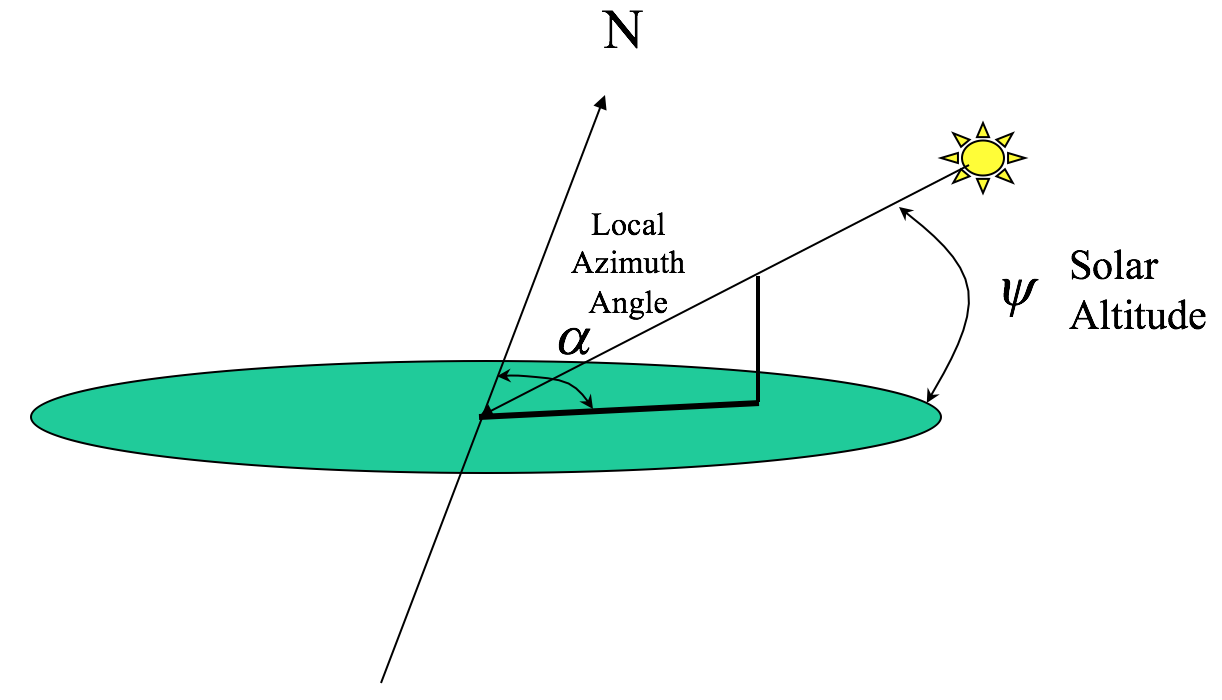
\includegraphics[width=1\textwidth]{fig5}\\
    \end{minipage}
    \end{column}
    \begin{column}{.5\textwidth}
    \begin{minipage}[c][0.65\textheight][c]{\linewidth}
   \begin{itemize}
   	\item $\psi$ - local sun elevation angle (``solar altitude'')
   	\item $\alpha$ - local azimuth angle \\($>0$ clockwise)
   	\item $\phi$ - latitude \\($>0$ N hemisphere)
   	\item $\lambda_e$ - longitude \\($>0$ W of prime meridian)
   \end{itemize}
      \end{minipage}
    \end{column}
  \end{columns}
\end{frame}
%------------------------------------------------
\begin{frame}{Radiation Model: Daily Effects}
\textbf{Spherical relationships for local elevation angle}
	$$\sin \psi = \sin \phi \sin \delta_s - \cos\phi\cos \delta_s \cos \underbrace{\left[\frac{Ct_{\text{UTC}}}{t_d} - \lambda_e\right]}_{B}$$
	where
	\begin{itemize}
		\item $C=360^\circ$ or $2\pi\ \radian$
		\item $t_{\text{UTC}} =$ local time + hours to UTC
		\item $t_d =$ 24 hours 
		\item $\lambda_e =$ longitude ($>0$ west from prime meridian)
	\end{itemize}
\end{frame}
%------------------------------------------------
\begin{frame}{Radiation Model: Daily Effects}
\textbf{Spherical relationships for local azimuth angle}
	$$\cos \alpha = \frac{\sin \delta_s - \sin \phi \cos \zeta}{\cos\phi \sin\zeta}$$
	where 
	\begin{itemize}
	\item the zenith angle $\zeta$ is given by
	\begin{align*}
	\zeta &= 90^\circ - \psi\\
	&= \frac{\pi}{2} - \psi\ (\text{radians})	
	\end{align*}
	\item Correction in afternoon for sun setting in west is
	$$\alpha^\prime = C-\alpha$$
	\end{itemize}
\end{frame}
%------------------------------------------------
\subsection{Slope Effects}
%------------------------------------------------
\begin{frame}{Radiation Model: Slope Effects}
\begin{figure}
	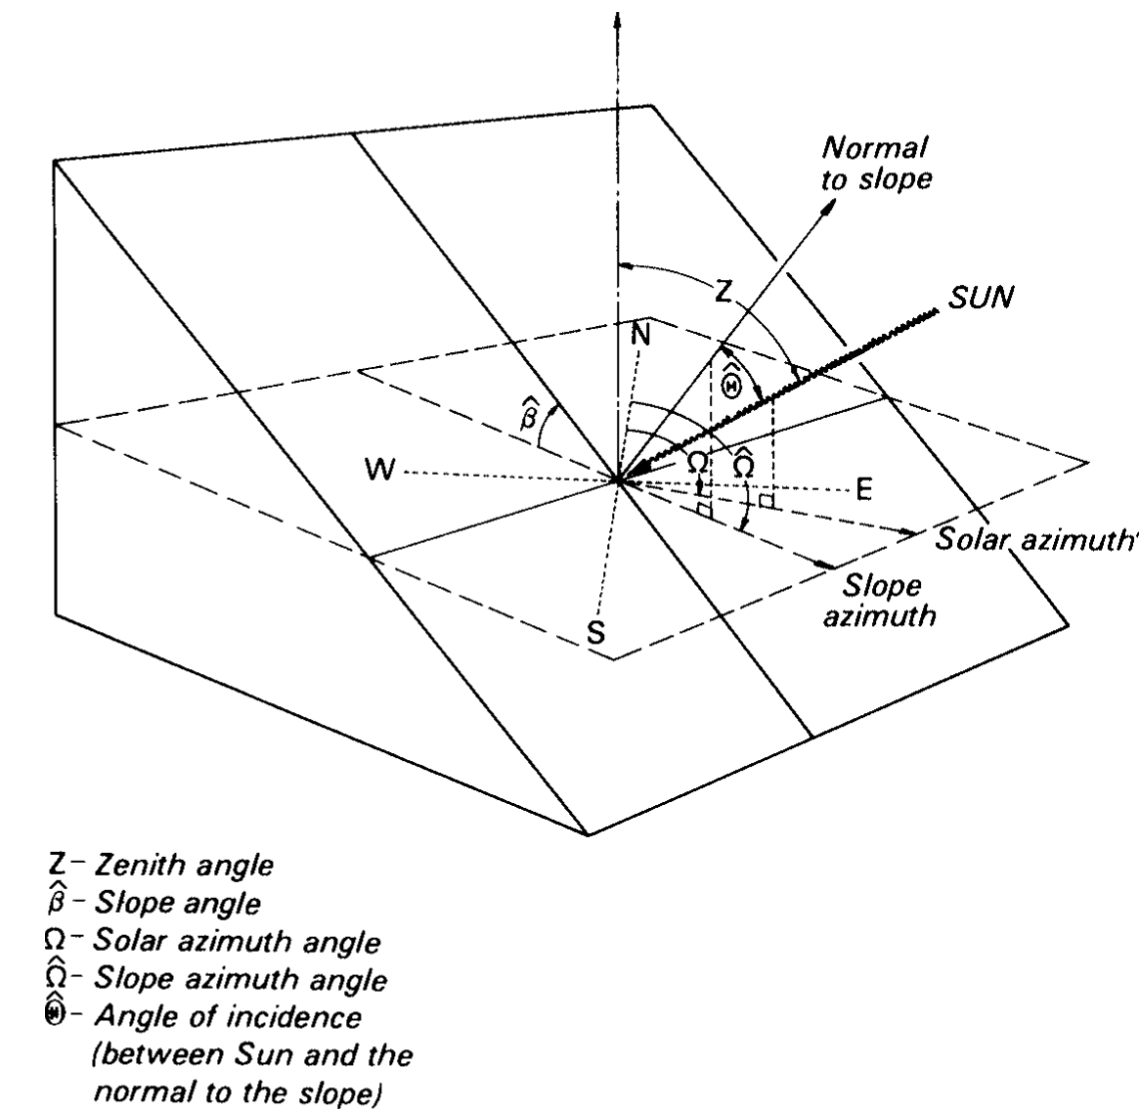
\includegraphics[width=0.78\textwidth]{fig6}
\end{figure}
\end{frame}
%------------------------------------------------
\begin{frame}{Radiation Model: Slope Effects}
\textbf{Spherical relationships for slope}
$$\cos \hat \theta = \cos \hat \beta \cos \zeta + \sin \hat \beta \sin \zeta \cos(\alpha - \hat \Omega)$$
Recall that for a flat surface
$$S=S_0 \cos \zeta$$
While for a sloping surface (absent scattering/absorption)
$$S=S_0 \cos \hat \theta$$
\end{frame}
%------------------------------------------------
\subsection{Net Shortwave}
%------------------------------------------------
\begin{frame}{Radiation Model: Net Shortwave}
\textbf{Net shortwave radiation}
$$R_s = R_{s\downarrow}(1-a)$$
if $|R_L|\ll R_s$ (true under clear skies during the day), then
$$R_N = R_{s\downarrow}(1-a)$$
In reality, we must also consider atmospheric transmissivity
\begin{align*}
	R_{s\downarrow} &= S_0 T_r \sin \phi\\
	&= S_0 T_r \cos \zeta
\end{align*}
where
\begin{itemize}
	\item $T_r =$ transmissivity (net sky transmissivity)
	\item $S_0 =$ solar constant $\simeq 1367\ \watt\ \metre\rpsquared$
\end{itemize}
\end{frame}
%------------------------------------------------
\begin{frame}{Radiation Model: Net Shortwave}
\textbf{Transmissivity}
Depends on 
\begin{itemize}
	\item path length through atmosphere
	\item atmospheric absorption
	\item cloudiness
\end{itemize}
Simple model
$$T_r = (0.6 + 0.2\sin \psi)(1-0.4\sigma_H)(1-0.7\sigma_M)(1-0.4\sigma_L)$$
where $\sigma_H$, $\sigma_M$, and $\sigma_L$ are cloud cover fractions for high-, mid-, and low-level clouds, respectively ($0 \leq \sigma_i \leq 1$)
\end{frame}
%------------------------------------------------
\subsection{Net Longwave}
%------------------------------------------------
\begin{frame}{Radiation Model: Net Longwave}
\textbf{Net longwave radiation}
$$R_L = R_{L\downarrow} + R_{L\uparrow}$$
where
$$R_{L\uparrow} = -\epsilon \sigma T^4$$
However, it is harder to model $R_{L\downarrow}$, so we will model the net longwave radiation $R_L$
$$R_L = b(1-0.1\sigma_H - 0.3\sigma_M-0.6\sigma_L)$$
where $b = -98.5\ \watt\ \metre\rpsquared$ 
\end{frame}
%------------------------------------------------
\subsection{Net Radiation Model}
%------------------------------------------------
\begin{frame}{Radiation Model: Net Radiation Model}
\textbf{Net radiation model}
\begin{align*}
	R_N &= R_{S\downarrow} + R_{S\uparrow} + R_{L\downarrow} + R_{L\uparrow}\\
	&= S_0Tr\cos\zeta(1-a) + R_L &\text{during day}&\\
	&= R_L (R_L<0) &\text{during night}&
\end{align*}
\end{frame}
%------------------------------------------------
\begin{frame}{Radiation Model: Net Radiation Model}
If asked to model $R_N$ for a specific location, on a specific day, at a specific time, with specific cloud cover and surface properties, follow these steps
\begin{itemize}
	\item Compute $\delta_s$
	\item Find solar elevation angle $\psi$
	\item Solve for transmissivity $T_r$
	\item Compute $R_S$ and $R_L$ contributions
	\item Compute $R_N$
\end{itemize}
\end{frame}

\end{document}

